\documentclass{examen}
\usepackage{listings}
\begin{document}

\modulo{Lenguajes de marcas -- PARTE ORDENADOR (PARTES 1 y 2)}

\pregunta{Crea una p�gina HTML que se modifique con CSS y que tenga un aspecto como el de la figura:
\begin{itemize}
\item{Se ha cambiado el tipo de letra de toda la p�gina, en concreto se ha usado el tipo Helvetica.}
\item{Observa que hay una lista en cuyos elementos han cambiado la vi�eta que aparece.}
\item{Hay una tabla con datos. Observa que la tabla tiene margen y que adem�s ciertas filas tienen cambiado el color de fondo (puedes poner el que quieras)}
\end{itemize}

}{2}
\begin{figure}[h]
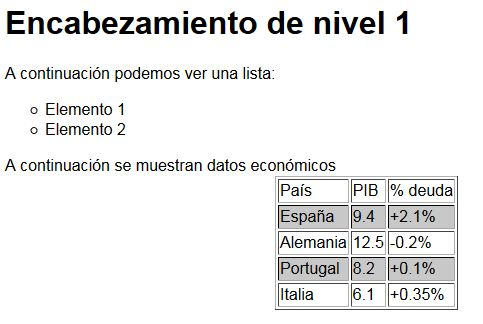
\includegraphics{examen-img/pagina.jpg}
\end{figure}

\break
\pregunta{Dado el archivo XML que se puede encontrar a continuaci�n, 
crear una hoja de estilo XSLT que transforme dicho archivo en el archivo XML que aparece al final. Recuerda que no hace falta escribir el fichero, en la herramienta JXMLTool podr�s insertar el fichero autom�ticamente usando el menu Ejemplos con la opci�n Inventario.
}{3}
\begin{verbatim}
<inventario><!--Archivo original-->
    <producto codigo="P1">
        <peso unidad="kg">10</peso>
        <nombre>Ordenador</nombre>
        <lugar edificio="B">
            <aula>10</aula>
        </lugar>
    </producto>
    <producto codigo="P2">
        <peso unidad='g'>500</peso>
        <nombre>Switch</nombre>
        <lugar edificio="A">
            <aula>6</aula>
        </lugar>
    </producto>
</inventario>
\end{verbatim}
\begin{verbatim}
<!--Esto debe ser lo que devuelva el archivo XSLT-->

<datos>
    <listacodigos>
        <codigo>P1</codigo>
        <codigo>P2</codigo>
    </listacodigos>
    <aulas>
        <aula>B-10</aula>
        <aula>A-6</aula>
    </aulas>
    <productos>
        <producto>
            Ordenador de 10kg
        </producto>
        <producto>
            Switch de peso 500g
        </producto>
    </productos>
</datos>

\end{verbatim}

\end{document}
